\documentclass{beamer}

\mode<presentation> {
\usetheme{Singapore}
}

\usepackage{graphicx}
\usepackage{booktabs} 

\usepackage{hyperref}
\usepackage{graphicx}
\graphicspath{ {images/} }
\usepackage{xcolor}

%----------------------------------------------------------------------------------------
%	TITLE PAGE
%----------------------------------------------------------------------------------------

\title[RL Methods]{Methods for solving
	continuous state and discrete action space 
	reinforcement learning problems} 


\begin{document}

\begin{frame}
\titlepage % Print the title page as the first slide
\end{frame}

\begin{frame}
\frametitle{Outline}

\tableofcontents 

\end{frame}

%----------------------------------------------------------------------------------------
%	PRESENTATION SLIDES
%----------------------------------------------------------------------------------------

%------------------------------------------------
\section{Introduction} 
%------------------------------------------------

\begin{frame}
\frametitle{Problem at Hand}
``Methods for solving
continuous state and discrete action space 
reinforcement learning problems'':

\begin{itemize}
\item Reinforcement Learning context -- trial-and-error search,
delayed rewards
\item Particular class of RL problems -- state is continuous,
action space is discrete 
\item Several methods -- we investigate what 
works: Random Agent, SARSA, Deep Q-Network 
\item Tested on OpenAI Lunar Lander environment
\item ``Solved'' when the trained agent obtains satisfactory 
performance (more than 200 points averaged over 100 runs)
\item Live demo!
\end{itemize}
\end{frame}


%------------------------------------------------

\begin{frame}
\frametitle{Motivation (General)}
\begin{block}{Different angle on existing problems}
Eg. Find shortest path in the maze, play chess, trade stocks. 
\end{block}

\begin{block}{New types of problems}
Eg. Play computer games, navigate a drone.
\end{block}

\begin{block}{Make use of a simulation environment}
Eg. Given an already developed 
simulator (General Mission Analysis Tool by NASA), 
create an autopilot 
for satellites.
\end{block}
\end{frame}

%------------------------------------------------

\begin{frame}
\frametitle{Motivation (Applications in NLP)}
\begin{block}{Article summarization}
	See ``A Deep Reinforced Model for Abstractive Summarization''
	by Xiong et al (\url{https://arxiv.org/abs/1705.04304}). 
\end{block}

\begin{block}{Question answering}
	Given a question q reformulate q to elicit the best possible answers. The agent seeks to
	find the best answer by asking many questions and aggregating the returned evidence (\url{https://arxiv.org/abs/1705.07830}).
\end{block}

\begin{block}{Text generation}
	Think of a dialogue as a sequential decision 
	making with each reply being a ``step''  (\url{https://arxiv.org/abs/1606.01541}).
\end{block}
\end{frame}

%------------------------------------------------

%------------------------------------------------
\section{Reinforcement Learning Overview}
%------------------------------------------------



\begin{frame}
\frametitle{Reinforcement Learning Problem}
\begin{itemize}
	\item Learning how to map situations to actions 
	\item Trial-and-error search
	\item Delayed feedback
	\item Trade-off between exploration and exploitation
	\item Sequential decision making
	\item Agent's actions affect the subsequent data it receives
\end{itemize}
\end{frame}

\begin{frame}
\frametitle{RL World}
\begin{columns}[c] 
	
	\column{.3\textwidth} % Left column and width
	\textbf{Components}:
	\begin{enumerate}
		\item State $S_t$
		\item Action $A_t(s)$
		\item Reward $R_t(s,a)$

		\item Policy $\pi(s)$
		\item Reward function $\mathcal{R}(s)$
		\item Value function $V(s)$

		\item Transition Function $Pr(s'|s,a)$
		\item Model

	\end{enumerate} 
	
	\column{.5\textwidth} % Right column and width
	\begin{figure}
		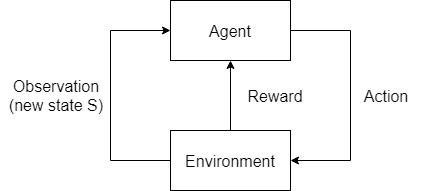
\includegraphics[scale=0.45]{rlw}
	\end{figure}
	
\end{columns}
\end{frame}


\begin{frame}
\frametitle{Definitions (1)}
\begin{itemize}
	\item Value function -- long-term ``value'' of a State $s$:	
	$$v_{\pi}(s)=\mathbb{E}_{\pi}\left[R_{t+1}+\gamma R_{t+2}+\gamma^{2} R_{t+3}+\ldots | S_{t}=s\right]$$
	
	
	\item Policy -- distribution over actions given states:
	$$
	\pi(a | s)=\mathbb{P}\left[A_{t}=a | S_{t}=s\right]
	$$
	
	
	\item Action-value function --  expected return
	starting from state $s$, taking action $a$, 
	and then following policy $\pi$:
	$$
	q_{\pi}(s, a)=\mathbb{E}_{\pi}\left[R_{t+1}+\gamma q_{\pi}\left(S_{t+1}, A_{t+1}\right) | S_{t}=s, A_{t}=a\right]
	$$
	
	After applying the Bellman equation

\end{itemize}
\end{frame}

\begin{frame}
\frametitle{Definitions (2)}

\begin{itemize}
	
	\item Optimal Value function -- maximum value
	function over all policies:	
$$
v_{*}(s)=\max _{\pi} v_{\pi}(s)
$$


\item Optimal Policy -- policy that ``beats''
any other policy:
$$
\pi_{*} \geq \pi, \forall \pi
$$
where
$$
\pi \geq \pi^{\prime} \text { if } v_{\pi}(s) \geq v_{\pi^{\prime}}(s), \forall s
$$

\end{itemize}

\end{frame}



\begin{frame}
\frametitle{Solutions to Our Problem Class}
\begin{columns}[c] % The "c" option specifies centered vertical alignment while the "t" option is used for top vertical alignment
	
	\column{.45\textwidth} % Left column and width
	\textbf{Characteristics}:
	\begin{itemize}
		\item Model is not known (no $\mathcal{R}$, no $\mathcal{P}$)
		\item State is continuous  
		\item Action space is discrete 
	
	\end{itemize} 
	
	\column{.45\textwidth} % Right column and width
		\textbf{Solutions}:
	\begin{itemize}
	\item Model-based: learn a model $\rightarrow$ solve MDP
	\item \textcolor{red}{Value-function based}: learn $Q$ $\rightarrow$ argmax
	\item Policy search: directly find $\pi$

	\end{itemize}
	
\end{columns}

\end{frame}


\begin{frame}
\frametitle{Model-free Value-function based methods}

\begin{itemize}
	\item Monte-Carlo RL
		\begin{itemize}
			\item from complete episode 
			\item episode must terminate
			\item unbiased
			\item high variance
		\end{itemize}
	
	\item Temporal-difference RL
		\begin{itemize}
			\item bootstrapping
			\item episode can be infinite
			\item biased
			\item lower variance
			\item faster convergence
		\end{itemize}
		
\end{itemize}
\end{frame}


\begin{frame}
\frametitle{Action Selection}

\begin{itemize}
	\item $\epsilon$-greedy (randomly selected action 
	with probability $\epsilon$, greedy otherwise)
	\item $\epsilon$-greedy with decay
	\item Softmax
$$
\pi(a)=\frac{\exp \left(\beta Q_{t}(a)\right)}{\sum_{a^{\prime} \in \mathcal{A}} \exp \left(\beta Q_{t}\left(a^{\prime}\right)\right)}
$$
	
	where $\beta$ > 0 controls the greediness of action selection
	($\beta \rightarrow \infty$ results in a greedy choice)
\end{itemize}
\end{frame}


\begin{frame}
\frametitle{SARSA Algorithm}

\begin{figure}
	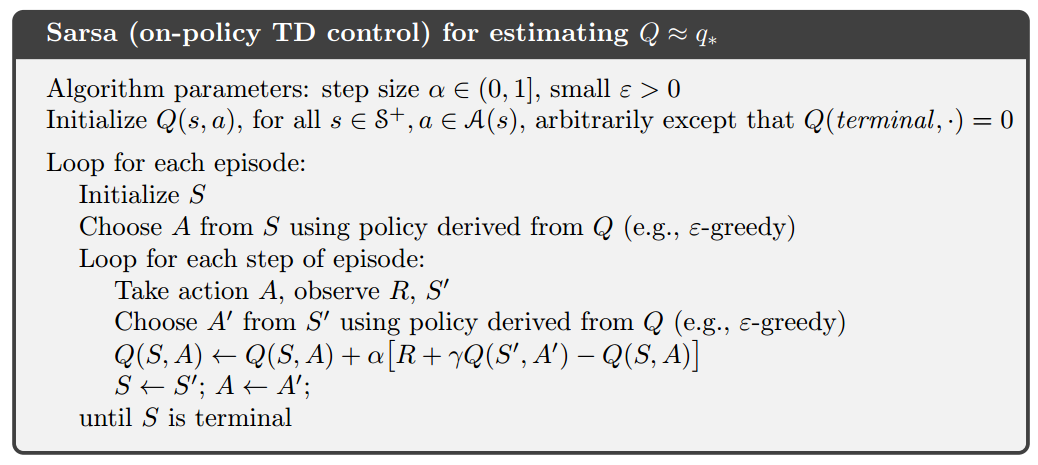
\includegraphics[scale=0.4]{sarsa}
\end{figure}

Source: Sutton

\end{frame}


\begin{frame}
\frametitle{Function Approximation}

Estimate value function with function approximation:

$$
\hat{v}(s, w) \approx v_{\pi}(s)
$$

Update $w$ with SGD $\rightarrow$ differentiable 
approximation functions:

$$
J(\mathbf{w})=\mathbb{E}_{\pi}\left[\left(v_{\pi}(S)-\hat{v}(S, \mathbf{w})\right)^{2}\right]
$$

$$
\Delta \mathbf{w} =-\frac{1}{2} \alpha \nabla_{\mathbf{w}} J(\mathbf{w})
 =\alpha \mathbb{E}_{\pi}\left[\left(v_{\pi}(S)-\hat{v}(S, \mathbf{w})\right) \nabla_{\mathbf{w}} \hat{v}(S, \mathbf{w})\right] 
$$

$$
\Delta \mathbf{w}=\alpha\left(v_{\pi}(S)-\hat{v}(S, \mathbf{w})\right) \nabla_{\mathbf{w}} \hat{v}(S, \mathbf{w})
$$

\end{frame}



%------------------------------------------------
\section{Solving the Lunar Lander Problem}
%------------------------------------------------

\subsection{Lunar Lander Environment}

\begin{frame}
\frametitle{Lunar Lander Environment}
\begin{columns}[c] % The "c" option specifies centered vertical alignment while the "t" option is used for top vertical alignment
	
	\column{.45\textwidth} % Left column and width
	OpenAI gym provides us with an interactive environment
	to control a robot. We have 8-D continuous 
	state space and action space of 4 discrete actions -- 
	do nothing, fire the left orientation engine, fire the main
	engine, fire the right orientation engine. 
	We are also controlling a robot during the flight. 
	
	\column{.5\textwidth} % Right column and width
	\begin{figure}
	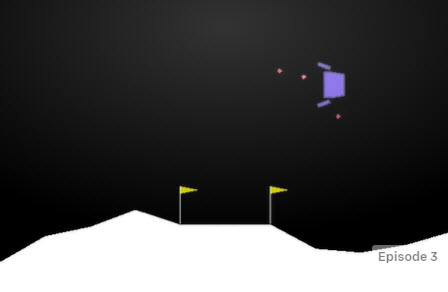
\includegraphics[scale=0.5]{lunar}
	\end{figure}
		
\end{columns}
\end{frame}


\begin{frame}
\frametitle{Experiment Design}
In order to reproduce and compare RL algorithms we devise 
a strict procedure for the experiments.
For each model we stick to the following workflow:

\begin{itemize}
	\item Run a training procedure for several ranges of episodes (eg. 100, 1000, 10000) and for several sets of hyper-parameters
	
	\item Analyze the trade-off between the running time and 
	model quality, select best-performing hyper-parameters
	
	\item Save the weights for best-performing hyper-parameters
	
	\item Load the weights and run a testing procedure for 100 episodes 
	
	\item Plot the score vs each testing episode
\end{itemize}

\end{frame}

\begin{frame}
\frametitle{Random Agent}
Random agent performance on 100, 1000 and 10000 episodes:

\begin{table}[H]
	\centering
	\begin{tabular}{|r|r|r|}
		\hline
		
		\multicolumn{1}{|l|}{\# Episodes} & \multicolumn{1}{l|}{Avg Training Score} & \multicolumn{1}{l|}{Last 100 Episodes} \\
		\hline
		100   & -175.399 & -175.399 \\
		\hline
		1000  & -175.124 & -197.221 \\
		\hline
		10000 & -182.212 & -172.897 \\
		\hline
	\end{tabular}%
	\label{tab:addlabel}%
\end{table}%



\end{frame}




\subsection{SARSA With Function Approximation}

\begin{frame}
\frametitle{SARSA Implementation}
The idea of the
algorithm is to approximate an action-value function Q(s, a) 
with a function Q(s, a, w) and to update a weight vector $w$
iteratively in the direction of the gradient:
\begin{equation}
\hat{q}(s, a, \mathbf{w}) = \mathbf{w}^{\top} \mathbf{x}(s, a)=\sum_{i=1}^{d} w_{i} \cdot x_{i}(s, a) 
\end{equation}

So that the gradient of the $\hat{q}(s, a, \mathbf{w})$ is:
\begin{equation}
\nabla \hat q(s,a,{\bf{w}}) = \nabla {\bf{w}}_{}^Tx(s,a) = x(s,a)
\end{equation}

With the update rule for weight vector:
\begin{equation}
{\bf{w}} \leftarrow {\bf{w}} + \alpha \left[ {R + \gamma \hat q\left( {{S^\prime },{A^\prime },{\bf{w}}} \right) - \hat q(S,A,{\bf{w}})} \right]x(s,a)
\end{equation}
\end{frame}



\begin{frame}
\frametitle{Empirical Results}
The best results were 
achieved with the learning rate of 0.1, gamma of 0.9 and 
exponential epsilon decay: 

\begin{table}[H]
	\centering
	\begin{tabular}{|r|r|r|}
		\hline
		\multicolumn{1}{|l|}{\# Episodes} & \multicolumn{1}{l|}{Avg Training Score} & \multicolumn{1}{l|}{Last 100 Episodes} \\
		\hline
		100   & -253.549 & -253.549 \\
		\hline
		1000  & -309.499 & -134.525 \\
		\hline
		10000 & -148.945 & -126.867 \\
		\hline
	\end{tabular}%
\end{table}%
\end{frame}


\begin{frame}
\frametitle{SARSA -- Conclusion}


\begin{itemize}
	\item Linear function approximation 
	cannot capture the complexity
	of the state landscape in the Lunar Lander case.
	
	\item To use 
	episodic semi-gradient Sarsa efficiently we need either 
	to define a more sophisticated non-linear approximation function or to 
	switch to another approach.

	\item Linear function approximation is compact. It takes 
	a vector of $n+m$ values to represent $w$. For the Lunar Lander problem parameter weights use 
	about 1 KB of disk space when saving with Python $joblib$ library.
	Other algorithms (as we will see with state discretization) can 
	require much more space.

\end{itemize}
\end{frame}







\subsection{Deep Q-Network}

\begin{frame}
\frametitle{Deep Q-Network Implementation (1)}
\begin{itemize}
	\item State is represented by a feature vector
	$\mathbf{x}(S)=\left(\begin{array}{c}{\mathbf{x}_{1}(S)} \\ {\vdots} \\ {\mathbf{x}_{8}(S)}\end{array}\right)$
	
	
	where the features are (x,y) coordinates, 
	velocity components on the x and y axes,
	angle of the lunar lander, angular
	velocity, binary values to indicate whether the left
	leg or right leg of the lunar lander is touching the ground	
\end{itemize} 
\end{frame}



\begin{frame}
\frametitle{Deep Q-Network Implementation (2)}
\begin{columns}[c] % The "c" option specifies centered vertical alignment while the "t" option is used for top vertical alignment
	
	\column{.45\textwidth} % Left column and width
	Approximator is an MLP of the 
	architecture
	8 x 500 x 200 x 100 x 4. Layers 
	are dense with relu activation. 
	
	\column{.5\textwidth} % Right column and width
	\begin{figure}
		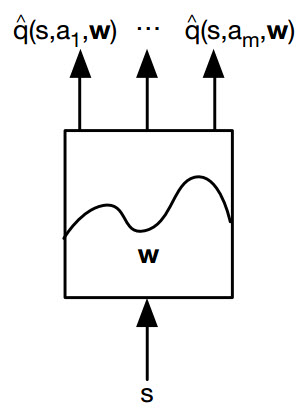
\includegraphics[scale=0.5]{nn}
	\end{figure}
	
\end{columns}
\end{frame}






\begin{frame}
\frametitle{Deep Q-Network Implementation (3)}
\begin{itemize}
	\item Approximate the action-value function
	
	\item Minimize MSE between approximate
	action-value function and true action-value function
	
	\item Use stochastic gradient descent to find a local minimum
	
	$\begin{aligned}-\frac{1}{2} \nabla_{\mathbf{w}} J(\mathbf{w}) &=\left(q_{\pi}(S, A)-\hat{q}(S, A, \mathbf{w})\right) \nabla_{\mathbf{w}} \hat{q}(S, A, \mathbf{w}) \\ \Delta \mathbf{w} &=\alpha\left(q_{\pi}(S, A)-\hat{q}(S, A, \mathbf{w})\right) \nabla_{\mathbf{w}} \hat{q}(S, A, \mathbf{w}) \end{aligned}$
	
	\item TD(0) is
	
	$\Delta \mathbf{w}=\alpha\left(R_{t+1}+\gamma \hat{q}\left(S_{t+1}, A_{t+1}, \mathbf{w}\right)-\hat{q}\left(S_{t}, A_{t}, \mathbf{w}\right)\right) \nabla_{\mathbf{w}} \hat{q}\left(S_{t}, A_{t}, \mathbf{w}\right)$
	
	
\end{itemize}
\end{frame}


\begin{frame}
\frametitle{Deep Q-Network Implementation in Keras}
DQN uses experience replay and fixed Q-targets:

\begin{itemize}
	\item Take action $a_t$ according to 
	$\epsilon$-greedy policy
	
	\item Store transition ($s_t$ , $a_t$ , $r_{t+1}$, $s_{t+1}$) 
	in replay memory $D$
	
	\item Sample random mini-batch of transitions ($s$, $a$, $r$, $s'$) from $D$
	
	\item Compute Q-learning targets w.r.t. old, fixed parameters $w^{-}$
	
	\item Optimize MSE between Q-network and Q-learning targets
	
	$\mathcal{L}_{i}\left(w_{i}\right)=\mathbb{E}_{s, a, r, s^{\prime} \sim \mathcal{D}_{i}}\left[\left(r+\gamma \max _{a^{\prime}} Q\left(s^{\prime}, a^{\prime} ; w_{i}^{-}\right)-Q\left(s, a ; w_{i}\right)\right)^{2}\right]$
	
	Using variant of stochastic gradient descent
		
\end{itemize}


Source: Silver; Mnih et al

\end{frame}


\begin{frame}
\frametitle{DQN Empirical Results}
The results after 1 million iterations (mean is 265): 

\begin{figure}
	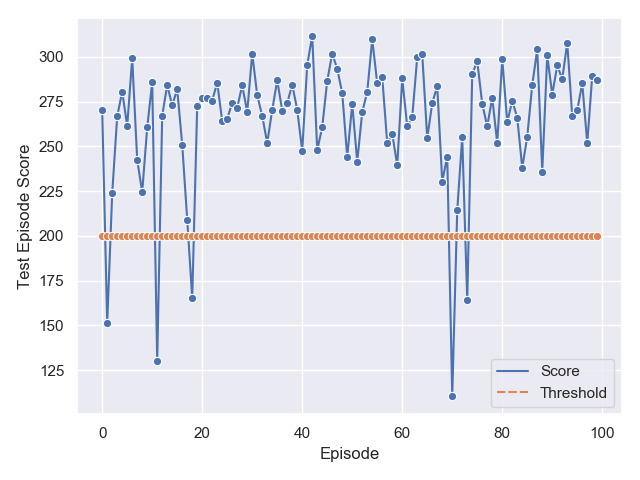
\includegraphics[scale=0.35]{nn_res}
\end{figure}

\end{frame}


\begin{frame}
\frametitle{DQN -- Conclusion}


\begin{itemize}
\item DQN is able to solve the Lunar Lander problem.

\item DQN takes longer time to converge (converged after 
1 million iterations).

\item Deep neural net approximation is not compact. 
In our case the network has over 100k of parameters. 
For the Lunar Lander problem parameter weights use 
about 512 KB of disk space when saving 
with Python $h5f$ library.

\end{itemize}
\end{frame}




\subsection{SARSA With State Discretization}

\begin{frame}
\frametitle{SARSA With State Discretization -- Implementation}
\begin{itemize}
	\item Initialize Q(s,a) table with 0 as a default 
	value for each state-action combination.
	
	\item After receiving a state from the environment, discretize it 
	using a binning approach.
	
	\item At each step take an $\epsilon$-greedy action -- random 
	with probability $\epsilon$ and 
	argmax(Q) with probability $1-\epsilon$.
	
	\item Compute the TD-target as
	\begin{equation}
	Target = R+\gamma Q\left(S^{\prime}, A^{\prime}\right)
	\end{equation}
	
	\item Compute the TD-error as
	\begin{equation}
	Error = Target - Q\left(S, A\right)
	\end{equation}	
	\item Update values of Q-table:
	\begin{equation}
	Q(S, A) \leftarrow Q(S, A)+\alpha Error
	\end{equation}		
\end{itemize} 
\end{frame}




\begin{frame}
\frametitle{Tuning Hyper-parameters}

\begin{block}{Feature dimensions}
	Setting the number of bins (dimensions) of 
	each state variable determines the size of the Q-table and the amount 
	of exploration we need to do. The number of discretized states grows 
	exponentially with the number of feature dimensions. 
\end{block}

\begin{block}{Alpha}
	Learning rate heavily influences the outcome of the 
	training process. Unlike neural nets, smaller alphas scored worse than 
	alphas of $0.1-0.2$.
\end{block}

\begin{block}{Epsilon}
	Several options are available: constant value, 
	exponential decay and piece-wise linear function.
\end{block}

\end{frame}

\begin{frame}
\frametitle{Tuning Hyper-parameters -- Alpha}
\begin{figure}[H]
	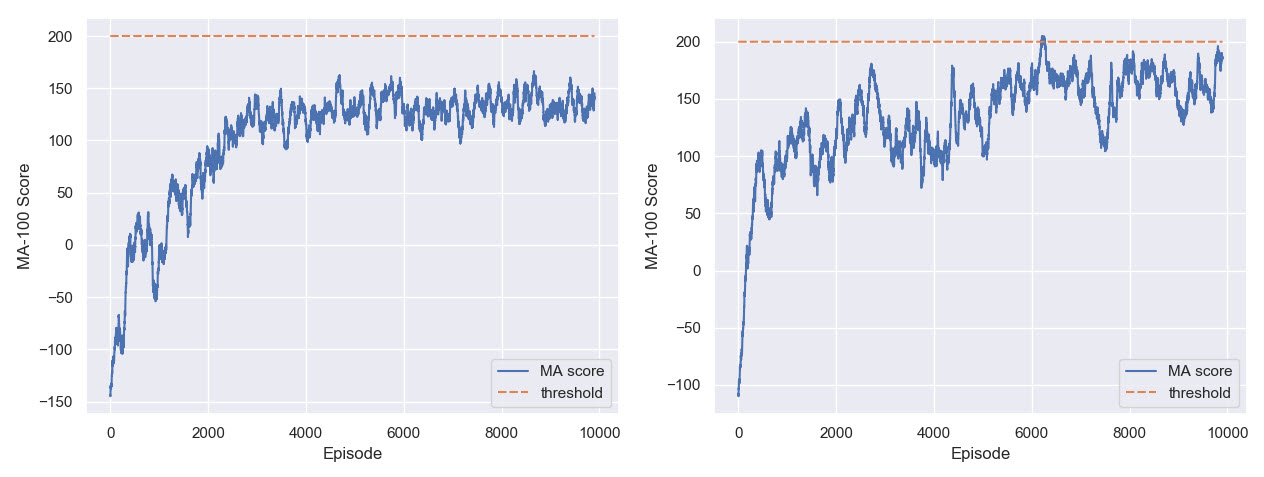
\includegraphics[scale=0.33]{a}
	\centering
	\caption{Training Scores For Alpha=0.05 (left) and Alpha=0.2 (right)}
	\label{f:a}
\end{figure}

\end{frame}


\begin{frame}
\frametitle{Training The Agent}
Training for 20,000 episodes, gamma=0.95,
alpha=0.2 and a piecewise linear epsilon schedule:

\begin{figure}[H]
	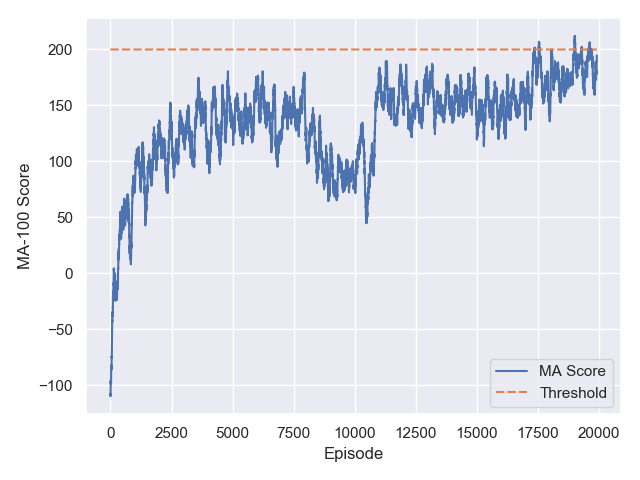
\includegraphics[scale=0.3]{train}
	\centering
	\caption{Moving Average-100 Training Scores For 20k Episodes}
	\label{f:train}
\end{figure}

\end{frame}

\begin{frame}
\frametitle{Testing The Agent}


\begin{figure}[H]
	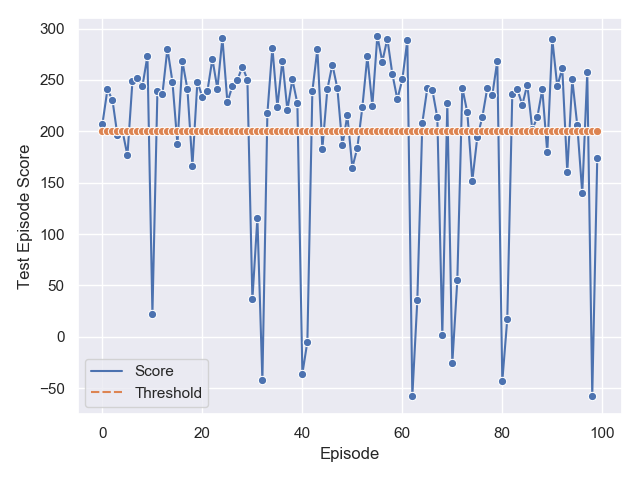
\includegraphics[scale=0.35]{test}
	\centering
	\caption{Testing Scores For 100 Episodes}
	\label{f:test}
\end{figure}
\end{frame}







%------------------------------------------------

\section{Conclusion}

\begin{frame}
\frametitle{Conclusion}
\begin{itemize}
	\item RL methods can be applicable to
	a wide variety of problems
	
	\item Out-of-the-box models work but 
	require fine-tuning and take 
	longer to converge
	
	\item Simple methods like state discretization
	are worth exploring when training speed and
	solution complexity are of the essence 
	
\end{itemize}
\end{frame}


\begin{frame}
\frametitle{References}
\footnotesize{
\begin{thebibliography}{5} 
	
\bibitem{rl1}\label{rl_book}
Reinforcement learning: an introduction, 2nd Edition. 
Richard S. Sutton, Andrew G. Barto. 

\bibitem{rl2}\label{ucl_course}
Reinforcement learning lectures by David Silver. UCL.
\url{http://www0.cs.ucl.ac.uk/staff/d.silver/web/Teaching.html} 

\bibitem{rl3}\label{deepmind}
Playing Atari with Deep Reinforcement Learning. Mnih et al.
\url{https://arxiv.org/abs/1312.5602}


\end{thebibliography}
}
\end{frame}

%------------------------------------------------

\begin{frame}

\begin{center}
	\Huge Thank you for 
	\\
	your attention!
\end{center}

\end{frame}

%----------------------------------------------------------------------------------------

\end{document}